\usetikzlibrary{decorations.markings, arrows, arrows.meta}

\tikzset{
    midar/.style={
        very thick,
        decoration={
            markings,
            mark=at position 0.55 with {\arrow{latex}}, % Arrow only at the midpoint
        },
        postaction=decorate,
    },
}

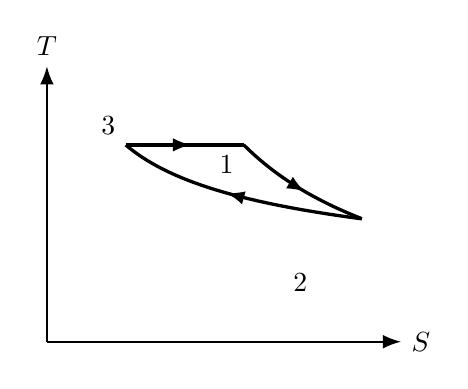
\begin{tikzpicture}[thick]
    % Shortened Axes
    \draw[-{Latex}] (0,0) -- (0,3.5) node[above] {$T$};
    \draw[-{Latex}] (0,0) -- (4.5,0) node[right] {$S$};

    % Points and labels
    \node at (1,2.5) [above left] {3};
    \node at (2.5,2.5) [below left] {1};
    \node at (3,1) [below right] {2};

    % Straight line from point 3 to point 1
    \draw[midar] (1,2.5) -- (2.5,2.5);

    % Hyperbolic curve from 3 to 1
    \draw[midar] plot[domain=2.5:4, samples=100] (\x, {6.25/\x});

    % Additional hyperbolic curve with specified domain
    \draw[midar] plot[domain=4:1, samples=100] (\x, {2.5/\x^0.34});
\end{tikzpicture}

